%                                                                    author:oh %
%%%%%%%%%%%%%%%%%%%%%%%%%%%%%%% Document Setup %%%%%%%%%%%%%%%%%%%%%%%%%%%%%%%%%
\documentclass[10pt]{article}

% Lorem ipsum
\usepackage{blindtext}
\newcommand{\shortlorem}{Lorem ipsum dolor sit amet, consectetuer adipiscing 
elit. Etiam lobortis facilisis sem. Nullam nec mi et neque pharetra 
sollicitudin. Praesent imperdiet mi nec ante. Donecullamcorper, felis non 
sodales commodo, lectus velit ultrices augue, a dignissim nibhlectus placerat 
pede. Vivamus nunc nunc, molestie ut, ultricies vel, semper in, velit.}

%Paper format 
\usepackage[paper=a4paper,
	hoffset=0mm,	        % Offset from left edge 
	marginparwidth=10mm,    % Width of margin
        marginparsep=0mm,       % Space between margin and main body
        margin=10mm,            % Margins
        includemp]{geometry}

\usepackage[T1]{fontenc}
\usepackage[utf8]{inputenc}

% Fonts
\usepackage{bookman}

% Figures
\usepackage{graphicx}
\graphicspath{ {./Latex/Figures} }

% Colors
\usepackage{color}
\usepackage{xcolor}

\definecolor{olofblue}{rgb}{0.486,0.647,0.8}
\definecolor{olofwhite}{rgb}{0.95,1,0.9}
\definecolor{olofgray}{rgb}{0.3,0.3,0.3}

% Graphics
\usepackage{tcolorbox}
\usepackage{worldflags}
\usepackage{etoolbox}
\usepackage{tikz}
\tcbuselibrary{skins}

% Date format
\usepackage{datetime}
\renewcommand{\dateseparator}{--}

% Arithmetic
\usepackage{calc}
\usepackage{pifont}
\usepackage{marvosym}

% Read data
\usepackage{readarray}

% Tables
\usepackage{tabularx}
\usepackage{paralist}
\usepackage[shortlabels]{enumitem}

% Page head, foot & numbering
\usepackage{fancyhdr}
\usepackage{lastpage}
\pagestyle{fancy}
\fancyhf{}
\fancyfoot[R]{\vspace{-10mm}Page \thepage \hspace{1pt} of \pageref{LastPage}}
\renewcommand{\headrulewidth}{0pt}

% Hyperlinks
\usepackage[unicode]{hyperref}
\hypersetup{colorlinks,breaklinks,
	linkcolor=black,urlcolor=olofblue,
        anchorcolor=olofblue,citecolor=olofblue}

%%%%%%%%%%%%%%%%%%%%%%%%%%%%%% Helper Commands %%%%%%%%%%%%%%%%%%%%%%%%%%%%%%%%%
% Custom symbol commands
\newrobustcmd*{\square}[1]{\tikz{\filldraw[draw=#1,fill=white] (0,0) 
	rectangle (2mm,2mm);}}

\newrobustcmd*{\filledsquare}[1]{\tikz{\filldraw[draw=#1,fill=#1] (0,0) 
	rectangle (2mm,2mm);}}

\newrobustcmd*{\filledcircle}[1]{\tikz{\filldraw[draw=#1,fill=#1] (0,0) circle (.5mm)
	node[anchor=center];}}

\newrobustcmd*{\lline}[1]{\tikz{\draw[draw=#1, thick] (0,0) -- (2mm,0) 
	node[anchor=left];}}

% Grading skills on a scale using custom symbols
\newcommand{\grade}[2]{%
	\newcounter{grading}
	\setcounter{grading}{1}
	\whiledo{\value{grading} < #2}{%
		\stepcounter{grading}
		}
}

% FOR EXAMPLE \grade{3}{6} should give a grade 3/6 of squares such that
% FS FS FS S S S
%
%

% Reading information variables from separate file
\newcommand\var[1]{\csname DATA#1\endcsname}
\readarraysepchar{=}
\readdef{./Config/varconfig.dat}{\data}
\readarray\data\MyDat[-,2]

\newcounter{datacount}%
\setcounter{datacount}{0}
\whiledo{\value{datacount} < \MyDatROWS}{%
	\stepcounter{datacount}%
	\expandafter\xdef\csname DATA\MyDat[\arabic{datacount},1]\endcsname{%
		\MyDat[\arabic{datacount},2]}%
}

% Head section
\newcommand{\makeheading}[1]%
	{\hspace{10mm - \marginparsep - \marginparwidth - \hoffset}%
	\begin{minipage}[t]{\textwidth}%
		{\fontsize{26}{0}\fontfamily{qbk}\selectfont #1}%
	\end{minipage}}

% Contact section
\newbox\contactbox
\newbox\mugshotbox
\newcommand{\makecontact}[8]%
	{\sbox\contactbox{
	\begin{minipage}[c]{.75\linewidth}
		\vspace{2mm}
		\fontsize{12}{0}\raggedright\textsc{Contact Information}
		\newlength{\rcollength}\setlength{\rcollength}{70mm}
	
		\vspace{2mm}
		\begin{tabular}[t]{@{}p{\textwidth-\rcollength}p{\rcollength}}
		#5, & \texttt{Phone}: \href{tel:#2}{#2}\\
		#6, & \texttt{E-mail}: \href{mailto:#3}{#3}\\
		#7  & \texttt{LinkedIn}: \href{#4}{#1}
		% add GitHub
		\end{tabular}
		\vspace{1mm}
	\end{minipage}}
	\newlength{\contactheight}\setlength{\contactheight}{2\ht\contactbox}
	
	\sbox\mugshotbox{
	\begin{minipage}[c]{\contactheight}
		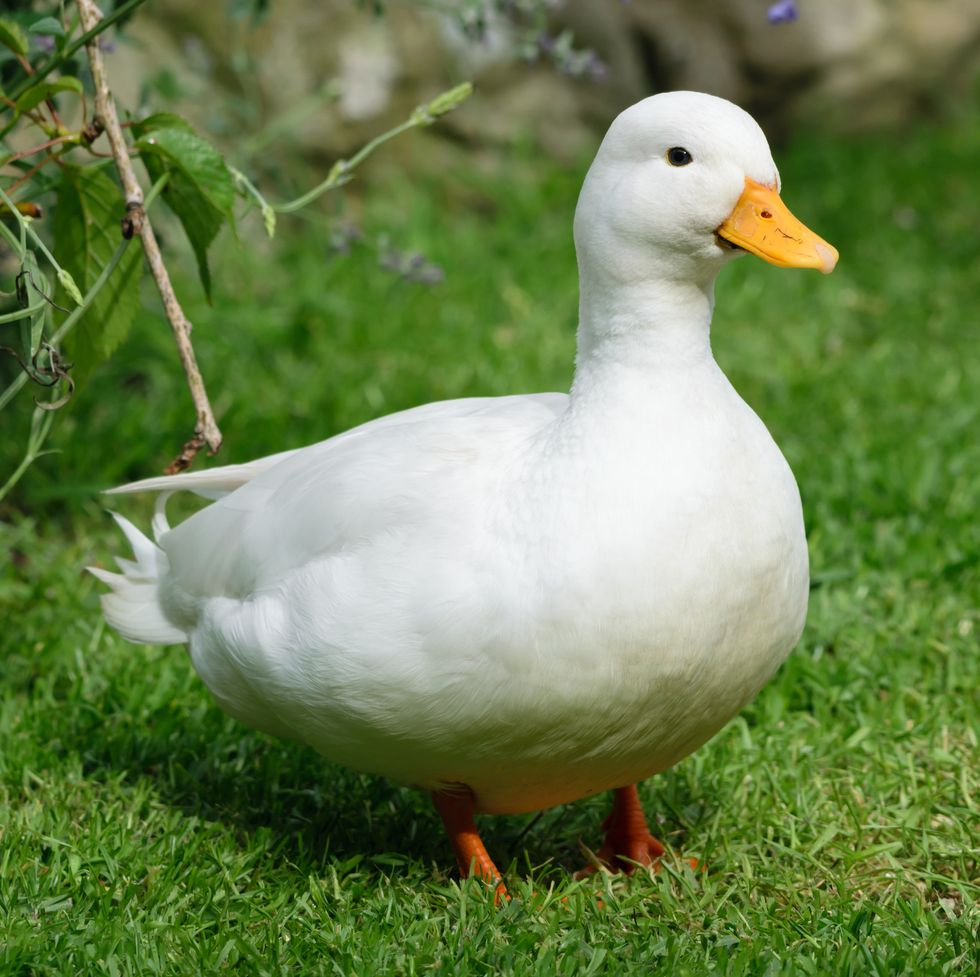
\includegraphics[width=\linewidth, height=\contactheight]{mugshot.png}
	\end{minipage}}
	\newlength{\mugshotwidth}\setlength{\mugshotwidth}{\wd\mugshotbox}
		
	\begin{minipage}{\linewidth - \mugshotwidth}	
		{\color{olofblue}\rule{\linewidth + 3pt}{.3pt}}

		\usebox\contactbox
		\begin{minipage}{.25\linewidth - \contactheight}
			\hfill
		\end{minipage}
	
		{\color{olofblue}\rule{\linewidth + 3pt}{.3pt}}
	\end{minipage}
	\begin{minipage}[c]{\mugshotwidth}
		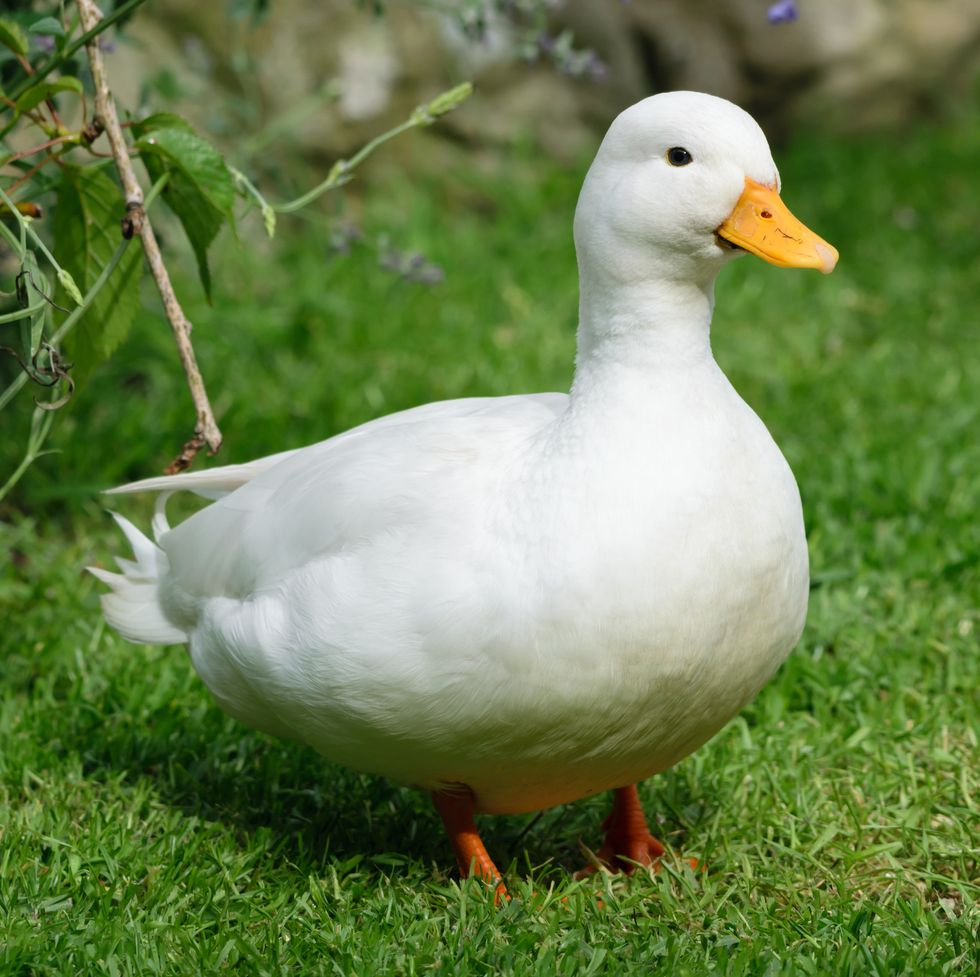
\includegraphics[width=.97\linewidth, height=.97\contactheight]{mugshot.png}
	\end{minipage}}

% Standard section - This would optimally be an enviromnent but I could not
%			get that to work.
\newcounter{sectioncounter}
\setcounter{sectioncounter}{0}
\newcommand{\makesection}[2]%
	{\pagebreak[2]\vspace{1mm}%

	\begin{minipage}{\linewidth}
	\begin{tcolorbox}[bicolor,            % Colorbox with two colors 
		sidebyside,		      % Two colorboxes side by side
		sidebyside gap=3mm,	      % Gap between colorboxes
		sidebyside align=top,         % Text alignment for both boxes
		lefthand width=.12\linewidth, % Width of left colorbox
		colback=olofblue,	      % Color background of first box
		colbacklower=white,           % Color background of second box
		colframe=white,               % Frame color
		colupper=olofwhite,           % Text color of first box
		sharp corners, 		      % Sharp box corners
		watermark graphics=wordcloud\thesectioncounter.png,
		watermark overzoom=1.5,
		watermark opacity=0.1, 
		width=\linewidth,             % Width of entire colorbox
		right=0mm,                    % Space between textbox and 
%right edge
		left=0mm,                     % Space between textbox and 
%left edge
		top=0mm                       % Space between textbox and 
%top edge
		]
	\addtocounter{sectioncounter}{1}
	%
	\fontsize{11}{0}\raggedright\scshape #1
	\tcblower
	#2
	\end{tcolorbox}
	\end{minipage}}

%%%%%%%%%%%%%%%%%%%%%%%%%%%%%% Define Variables %%%%%%%%%%%%%%%%%%%%%%%%%%%%%%%%
% Semi-Permanent

\def\myname{\var{myname}}
\def\phone{\var{myphone}}
\def\email{\var{mymail}}
\def\linkedin{\var{mywebsite}}
\def\myadress{\var{myadress}}
\def\mycity{\var{mycity}}
\def\mycountry{\var{mycountry}}

%%%%%%%%%%%%%%%%%%%%%%%%%%%%%%% Begin Document %%%%%%%%%%%%%%%%%%%%%%%%%%%%%%%%%
\begin{document}

%% ======================================= HEAD
\makeheading{\myname}

%% ======================================= CONTACT
\makecontact{\myname}{\phone}{\email}{\linkedin}{\myadress}{\mycity}{\mycountry}

%% ======================================= ABOUT ME
\makesection{About Me}{\shortlorem}

%% ======================================= WORK EXPERIENCE
\makesection{Work Experience}{%
	{\fontsize{11}{10}\textsc{SmallCorp}}
	\hfill 20XX-20XX

		{\small I worked X years at SmallCorp in a consultancy role to the assistant supervisor. During these years I learned of the value hard work can have on ur profit margins. I also got learned alot about the best way to get your way.}\\
	
	{\fontsize{11}{10}\textsc{CityCorp}}
	\hfill 20XX-20XX

		{\small For X years I worked with pushing pencils at my local CityCorp office. Here I learned such important skills as the optimal coffee temperature and why you should never have onion with mayonaise. I also learned significantly about what is going on.}}
    
%% ======================================= EDUCATION
\makesection{Education}{%
	{\fontsize{11}{10}\textsc{Practical U}}
	\hfill 20XX-20XX
        \begin{itemize}[leftmargin=5mm, itemsep=2mm, parsep=0mm]
        	\item[\filledcircle{olofblue}] Certificate of Approval in Microwave Management
	\end{itemize}

	{\fontsize{11}{10}\textsc{Big U}}
	\hfill 20XX-20XX
        \begin{itemize}[leftmargin=5mm, itemsep=2mm, parsep=0mm]
        	\item[\filledcircle{olofblue}] {\textit{PhD}} in Philosophy
        	\begin{itemize}
			\item[] Thesis: \textit{What is going on?}
       		\end{itemize}
	\end{itemize}
	
	{\fontsize{11}{10}\textsc{City U}}
	\hfill 20XX-20XX
        \begin{itemize}[leftmargin=5mm, itemsep=2mm, parsep=0mm]
        	\item[\filledcircle{olofblue}] {\textit{MSc}} in Waste Management
        	\begin{itemize}
			\item[] Thesis: \textit{Causes and effects of contracyclical waste gathering on \\asymmetrical behavioural dependencies in rats.}
       		\end{itemize}
	\end{itemize}}

%% ======================================= SOFTWARE SKILLS
\makesection{Software Skills}{% 
	\begin{itemize}[leftmargin=5mm, itemsep=2mm, parsep=0mm]
		\item[\lline{olofblue}] {\fontsize{11}{0}\textsc{Computer}}
			
			{\small Excellent computer skills. Unparallelled even.} 
    

        	\item[\lline{olofblue}] {\fontsize{11}{0}\textsc{Xbox}}

			{\small I have played on the xbox platform for about 14 years and is thus very experienced with using an xbox.} 

	\end{itemize}}

%% ======================================= PRACTICAL SKILLS
\makesection{Practical Skills}{%
	\begin{itemize}[leftmargin=5mm, itemsep=2mm, parsep=0mm]
        	\item[\lline{olofblue}] {\fontsize{11}{0}\textsc{Microwave}}

			{\small I know how to operate most microwaves and have even obtained a certificate in microwave management at Practical U.} 
            
        	\item[\lline{olofblue}] {\fontsize{11}{0}\textsc{Tie Shoe}}

			{\small Personal record at 3.42 seconds and I know 17 different shoe tie knots.}

	\end{itemize}}

%% ======================================= OTHER SKILLS
\makesection{Other Skills}{%
{\fontsize{12}{10}\textsc{Languages}} 

\vspace{3mm}
\begin{minipage}{\linewidth}
\begin{tabularx}{\linewidth}{ >{\raggedright}X >{\raggedright}X }
        \worldflag[width=3mm]{PL} \fontsize{11}{10}\textsc{Polish} &
	\worldflag[width=3mm]{KR} \fontsize{11}{10}\textsc{Korean} & 
	\filledsquare{olofblue} \filledsquare{olofblue} \filledsquare{olofblue}
	\filledsquare{olofblue} \filledsquare{olofblue} \filledsquare{olofblue} &
	\filledsquare{olofblue} \filledsquare{olofblue} \filledsquare{olofblue}
	\square{olofblue} \square{olofblue} \square{olofblue} &
	\grade{6}{6} &
	\grade{3}{6}
\end{tabularx}
\end{minipage}}

\end{document}

